\section{The Structure of Sets}
    We've developed two \textit{operations}\index{Binary Operation} on sets thus
    far, those of union and intersection. Several of their properties give rise
    to the notion of a \textit{Boolean algebra}\index{Boolean Algebra}. Many
    theorems about sets can then be proven algebraically and it is our current
    goal to prove the basics about unions and intersections so we may transition
    to algebra.
    \subsection{Basic Theorems}
        With the law of the excluded middle established we may now rapidly prove
        many basic results about sets. First, we prove the empty set is unique.
        \begin{theorem}
            \label{thm:Emptyset_Is_Subset}%
            If $A$ is a set, then $\emptyset\subseteq{A}$.
        \end{theorem}
        \begin{proof}
            For if not, then there is an $x\in\emptyset$ such that
            $x\notin{A}$ (Def.~\ref{def:Subsets}). But for all $x$ it is true
            that $x\notin\emptyset$ (Def.~\ref{def:Empty_Set}), a contradiction.
            Therefore $\emptyset\subseteq{A}$.
        \end{proof}
        \begin{theorem}
            \label{thm:Empty_Set_is_Unique}%
            If $\emptyset'$ is a set with no elements, then
            $\emptyset=\emptyset'$.
        \end{theorem}
        \begin{proof}
            For suppose not. But $\emptyset'$ is a set, and thus
            $\emptyset\subseteq\emptyset'$ (Thm.~\ref{thm:Emptyset_Is_Subset}).
            By the definition of equality if $\emptyset\ne\emptyset'$,
            then $\emptyset'\nsubseteq\emptyset$ (Def.~\ref{def:Equal_Sets}).
            But then there is an $x$ such that $x\in\emptyset'$ and
            $x\notin\emptyset$ (Def.~\ref{def:Subsets}). But by hypothesis
            $\emptyset'$ contains no elements, a contradiction. Thus
            $\emptyset'\subseteq\emptyset$. Therefore, $\emptyset=\emptyset'$
            (Def.~\ref{def:Equal_Sets}).
        \end{proof}
        With this we can define \textit{the} empty set.
        \begin{fdefinition}{The Empty Set}{Empty_Set}
            The \gls{empty set} is the unique \gls{set} $\emptyset$ such that
            for all $x$ it is true that $x\notin\emptyset$.\index{Empty Set}
        \end{fdefinition}
        Often times when encountering problems with sets, or in any other branch
        of mathematics, one creates a chain of equalities or inequalities and
        then invokes the \textit{transitive law} to conclude the proof. Such
        examples are found in elementary arithmetic with real numbers: If $a<b$
        and $b<c$, for real numbers $a,b,c\in\mathbb{R}$, then it must be true
        that $a<c$. Similar claims are found in Euclidean geometry. Indeed, if
        one were to peruse book one of Euclid's
        \textit{Elements}\index{Elements, Euclid's}, common notion 1 reads:
        \textit{things which are equal to the same thing are also equal to one
        another}. That is, if $A=B$ and if $B=C$, then $A=C$. Euclid adopted
        this as a fundamental truth, or \textit{axiom}, the word
        \textit{equality} being one of his primitive undefined words. We've used
        the language of sets and thus the transitivity of equality must be
        proved as a theorem using the definitions adopted. To do so first
        requires the transitivity of inclusion, since equality is defined in
        terms of subsets.
        \begin{ltheorem}{Transitivity of Inclusion}{Transitivity_of_Inclusion}
            If $A$, $B$, and $C$ are sets, if $A\subseteq{B}$, and if
            $B\subseteq{C}$, then $A\subseteq{C}$.\index{Relation!Transitive}
            \index{Transitivity!of Inclusion}
        \end{ltheorem}
        \begin{proof}
            For suppose not. Then by the definition of subset there is an
            $x\in{A}$ such that $x\notin{C}$ (Def.~\ref{def:Subsets}). But $A$
            is a subset of $B$ and thus $x\in{B}$ (Def.~\ref{def:Subsets}).
            Similarly, $B$ is a subset of $C$ and therefore $x\in{C}$
            (Def.~\ref{def:Subsets}), a contradiction.
        \end{proof}
        \begin{example}
            Consider the sets we've discussed so far: $\mathbb{N}$,
            $\mathbb{Z}$, and $\mathbb{Q}$. We can see from
            Eqns.~\ref{eqn:Natural_Numbers_Ellipses} and
            \ref{eqn:Integers_Ellipses} that $\mathbb{N}\subseteq\mathbb{Z}$,
            and we've also claimed that $\mathbb{Z}\subseteq\mathbb{Q}$. By the
            transitivity of inclusion (Thm.~\ref{thm:Transitivity_of_Inclusion})
            we then have $\mathbb{N}\subseteq\mathbb{Q}$.
        \end{example}
        Containment (\gls{containmentsymb}) is not transitive. That is, if
        $A\in{B}$ and $B\in{C}$, it may not be true that $A\in{C}$, nor is it
        necessarily true that $\{A\}\in{C}$, or even $\{A\}\subseteq{C}$. For a
        simple example, let $A=\emptyset$, $B=\{A,\{A\}\}$, and
        $C=\{B\}$. Then by definition $A\in{B}$ and $B\in{C}$, but $A\notin{C}$.
        This is because for all $x$ it is true that $x\in{C}$ if and only if
        $x=B$, and since $A\in{B}$ it is necessarily true that $A\ne{B}$
        (see Thm.~\ref{thm:Containment_NEqual_Underlying_Set}), and therefore
        $A\notin{C}$. Moreover, since $\{A\}\notin\{A\}$
        (Thm.~\ref{thm:Anti_Russells_Paradox}) and $\{A\}\in{B}$, by the axiom
        of extensionality (Ax.~\ref{ax:Axiom_of_Extensionality}) we conclude
        that $\{A\}\ne{B}$. Thus $\{A\}\notin{C}$ and $\{A\}\nsubseteq{C}$. This
        last claim stems from the fact that the only subsets of $C$ are
        $\emptyset$ and the entirety of $C$ itself. But
        $\emptyset\ne\{\emptyset\}$ and $\{\emptyset\}\ne{C}$, and thus
        $\{A\}\nsubseteq{C}$.
        \par\hfill\par
        It is possible to find sets $A$, $B$, and $C$ such that $A\in{B}$,
        $B\in{C}$, and $A\in{C}$, we need only consider a nested chain of sets.
        Let $A=\emptyset$, $B=\{\emptyset\}$, and
        $C=\{\emptyset,\{\emptyset\}\}$. We can write this more clearly as
        follows:
        \par
        \begin{subequations}
            \begin{minipage}[b]{0.32\textwidth}
                \centering
                \begin{equation}
                    A=\emptyset
                \end{equation}
            \end{minipage}
            \hfill
            \begin{minipage}[b]{0.32\textwidth}
                \centering
                \begin{equation}
                    B=\{\,A\,\}
                \end{equation}
            \end{minipage}
            \hfill
            \begin{minipage}[b]{0.32\textwidth}
                \centering
                \begin{equation}
                    C=\{\,A,\,B\,\}
                \end{equation}
            \end{minipage}
        \end{subequations}
        \par\vspace{2.5ex}
        Then by construction, $A\in{B}$, $B\in{C}$, and $A\in{C}$. Such chains
        are used in the von Neumann\index{von Neumann, John} construction of the
        integers.
        \par\hfill\par
        With the transitivity of inclusion we can present a few brief
        corollaries.
        \begin{theorem}
            \label{thm:Subsets_of_Equal_Sets}%
            If $A$, $B$, and $C$ are sets, if $A=B$, and if $C\subseteq{A}$,
            then $C\subseteq{B}$.
        \end{theorem}
        \begin{proof}
            For if $A=B$, then $A\subseteq{B}$ (Def.~\ref{def:Equal_Sets}). But
            by the transitivity of inclusion, if $C\subseteq{A}$ and
            $A\subseteq{B}$, then $C\subseteq{B}$
            (Thm.~\ref{thm:Transitivity_of_Inclusion}).
        \end{proof}
        This theorems relates subsets and equal sets, and in a similar manner
        we can relate \textit{supersets}. A superset of a set $A$ is simply a
        set $B$ that contains $A$. That is, $A\subseteq{B}$. This is the dual
        notion of a subset.
        \begin{theorem}
            \label{thm:Superset_of_Equal_Sets}%
            If $A,B$, and $C$ are sets, if $A=B$, and if $A\subseteq{C}$, then
            $B\subseteq{C}$.
        \end{theorem}
        \begin{proof}
            For if $A=B$ then $B\subseteq{A}$ (Def.~\ref{def:Equal_Sets}).
            But if $B\subseteq{A}$ and $A\subseteq{C}$, then by the transitivity
            of inclusion, $B\subseteq{C}$
            (Thm.~\ref{thm:Transitivity_of_Inclusion}).
        \end{proof}
        More than just being transitive, inclusion is also reflexive.
        \begin{ltheorem}{Reflexivity of Inclusion}{Reflexivity_of_Inclusion}
            If $A$ is a set, then $A\subseteq{A}$.
            \index{Relation!Reflexive}\index{Reflexivity!of Inclusion}
        \end{ltheorem}
        \begin{proof}
            For if not, then by the definition of subset there is an $x\in{A}$
            such that $x\notin{A}$ (Def.~\ref{def:Subsets}), a contradiction.
            Therefore $A\subseteq{A}$.
        \end{proof}
        The notion of inclusion (\gls{subseteq}) is also
        antisymmetric\index{Relation!Antisymmetric}. That is to say, if
        $A\subseteq{B}$ and $B\subseteq{A}$, then $A=B$. This is simply the
        definition of equality (Def.~\ref{def:Equal_Sets}). A relation that is
        transitive, reflexive, and antisymetric is known as a partial
        ordering\index{Partial Order}. The partial ordering of inclusion on the
        power set of some given set is the quintessential example of a partial
        order. On the other hand, the notion of containment is not reflexive.
        That is, for any set $A$ it is true that $A\notin{A}$
        (Thm.~\ref{thm:Anti_Russells_Paradox}). Indeed, this is desired to avoid
        Russell's Paradox\index{Russell's Paradox}. We now turn towards proving
        the familiar structure behind the notion of equality.
        \begin{ltheorem}{Reflexivity of Equality}{Equality_Reflexive}
            If $A$ is a set, then $A=A$.
            \index{Relation!Reflexive}\index{Reflexivity!of Equality}
        \end{ltheorem}
        \begin{proof}
            For if $A$ is a set then $A\subseteq{A}$
            (Thm.~\ref{thm:Reflexivity_of_Inclusion}). Thus, $A=A$
            (Def.~\ref{def:Equal_Sets}).
        \end{proof}
        And equally trivial theorem is the symmetry of equality, a direct
        corollary of the commutativity of the disjunction connective
        (\gls{conjunctionsymb}).
        \begin{ltheorem}{Symmetry of Equality}{Symmetry_of_Equality}
            If $A$ and $B$ are sets and if $A=B$, then $B=A$.
            \index{Relation!Symmetric}\index{Symmetry!of Equality}
        \end{ltheorem}
        \begin{proof}
            For if $A=B$, then $A\subseteq{B}$ and $B\subseteq{A}$
            (Def.~\ref{def:Equal_Sets}). But then
            $B\subseteq{A}$ and $A\subseteq{B}$, and thus $B=A$
            (Def.~\ref{def:Equal_Sets}).
        \end{proof}
        An important but non-obvious statement is that containment
        (\gls{containmentsymb}) is \textit{not} symmetric, and indeed is the
        exact opposite, it is antisymetric. That is, for any two sets $A$ and
        $B$ it impossible for both $A\in{B}$ and $B\in{A}$, for this would
        violate the axiom of regularity\index{Axiom!of Regularity}
        (Ax.~\ref{ax:Axiom_of_Regularity}). We now prove this claim rigorously.
        \begin{ltheorem}{Antisymmetry of Containment}
                        {Antisymmetry_of_Containment}
            If $A$ and $B$ are sets, and if $A\in{B}$, then $B\notin{A}$.
            \index{Relation!Antisymmetric}\index{Antisymmetry!of Containment}
        \end{ltheorem}
        \begin{proof}
            For suppose not, and suppose $B\in{A}$. But by
            Thm.~\ref{thm:Existence_of_Set_Built_from_Two_Sets}, if $A$ and $B$
            are sets, then there is a set $\{A,B\}$ such that for all $x$ it is
            true that $x\in\{A,B\}$ if and only if $x=A$ or $x=B$. But then
            $\{A,B\}$ is a non-empty set, and thus by the axiom of regularity
            (Ax.~\ref{ax:Axiom_of_Regularity}) there is an $x\in\{A,B\}$ such
            that $x\cap\{A,B\}=\emptyset$. But by hypothesis, $A\in{B}$, and
            thus $A\in{B}\cap\{A,B\}$ (Def.~\ref{def:Intersection_of_Two_Sets}),
            and therefore $x\ne{B}$. But similarly, if $B\in{A}$, then
            $B\in{A}\cap\{A,B\}$ and thus $x\ne{A}$. But $x\in\{A,B\}$ if and
            only if $x=A$ or $x=B$, a contradiction. Therefore, $B\notin{A}$.
        \end{proof}
        An instant corollary of this is that $\{A\}\notin{A}$.
        \begin{theorem}
            \label{thm:Set_Containing_A_is_not_Element_of_A}%
            If $A$ is a set, then $\{A\}\notin{A}$.
        \end{theorem}
        \begin{proof}
            For $A\in\{A\}$ (Thm.~\ref{thm:Existence_of_Set_Containing_Set}).
            But if $A\in\{A\}$, then $\{A\}\notin{A}$
            (Thm.~\ref{thm:Antisymmetry_of_Containment}).
        \end{proof}
        We now continue developing the structure of equality.
        \begin{ltheorem}{Transitivity of Equality}{Transitivity_of_Equality}
            If $A$, $B$, and $C$ are sets, if $A=B$, and if $B=C$, then $A=C$.
        \end{ltheorem}
        \begin{proof}
            For if $B=C$, then $C\subseteq{B}$ (Def.~\ref{def:Equal_Sets}). But
            if $A=B$, then $B=A$ (Thm.~\ref{thm:Reflexivity_of_Inclusion}). But
            if $B=A$ and $C\subseteq{B}$, then $C\subseteq{A}$
            (Thm.~\ref{thm:Subsets_of_Equal_Sets}). And if $A=B$, then
            $A\subseteq{B}$ (Def.~\ref{def:Equal_Sets}). But if $B=C$ and
            $A\subseteq{B}$, then $A\subseteq{C}$
            (Thm.~\ref{thm:Subsets_of_Equal_Sets}). But it was proved that
            $C\subseteq{A}$, and thus $A=C$ (Def.~\ref{def:Equal_Sets}).
        \end{proof}
        The three properties we've proved thus far, that of reflexivity
        (Thm.~\ref{thm:Equality_Reflexive}), symmetry
        (Thm.~\ref{thm:Symmetry_of_Equality}), and transitivity
        (Thm.~\ref{thm:Transitivity_of_Equality}), are the key ingredients in
        defining \textit{equivalence relations}\index{Equivalence Relation}.
        These are relations which are used to model the notion of equality in
        more abstract setting. We'll discuss these more in
        \S~\ref{Section:ZFC:Elementary_Set_Theory:Relations}.
        \begin{theorem}
            \label{thm:Prop_Subset_Not_Equal}%
            If $A$ and $B$ are sets, and if $A\subsetneq{B}$, then there is an
            $x\in{B}$ such that $x\notin{A}$.
        \end{theorem}
        \begin{proof}
            For suppose not. Then for all $x\in{B}$ it is true that $x\in{A}$.
            But then $B\subseteq{A}$ (Def.~\ref{def:Subsets}).
            But $A\subseteq{B}$ and thus $A=B$ (Def.~\ref{def:Equal_Sets}).
            But $A\subsetneq{B}$ and therefore $A\ne{B}$, a contradiction.
        \end{proof}
        \begin{theorem}
            If $A$ is a set, then $A$ is not a proper subset of $\emptyset$.
        \end{theorem}
        \begin{proof}
            For suppose not. Then there is an $x\in\emptyset$ such that
            $x\notin{A}$ (Thm.~\ref{thm:Prop_Subset_Not_Equal}), a
            contradiction (Def.~\ref{def:Empty_Set}).
        \end{proof}
    \subsection{Operations on Sets}
        Similar to the arithmetic of real numbers, there are standard operations
        that can be performed on sets to obtain new sets. The four most common
        operations are union, intersection, set difference, and symmetric
        difference. As stated before, we wish to build the structure of sets in
        an algebraic manner. To do this requires the notion that the operations
        of intersection and unions are \textit{commutative},
        \textit{distributive}, have \textit{identities}, and have
        \textit{complements}.
        \begin{ltheorem}{Commutative Law of Unions}{Commutative_Law_of_Unions}
            If $A$ and $B$ are sets, then $A\cup{B}=B\cup{A}$.
            \index{Commutative Law!of Unions}
        \end{ltheorem}
        \begin{proof}
            For if $x\in{A}\cup{B}$, then either $x\in{A}$ or $x\in{B}$, or both
            (Def.~\ref{def:Union_of_Two_Sets}). But then either $x\in{B}$ or
            $x\in{A}$, or both, and therefore $x\in{B}\cup{A}$
            (Def.~\ref{def:Union_of_Two_Sets}). But then for all
            $x\in{A}\cup{B}$ it is true that $x\in{B}\cup{A}$, and therefore
            $A\cup{B}\subseteq{B}\cup{A}$ (Def.~\ref{def:Subsets}). Similarly,
            $B\cup{A}\subseteq{A}\cup{B}$, and thus
            $A\cup{B}=B\cup{A}$ (Def.~\ref{def:Equal_Sets}).
        \end{proof}
        Taking unions tends to produce \textit{larger} sets, a property that is
        analogous to the addition of non-negative real numbers. Given any such
        values $a,b\geq{0}$ it is true that $a\leq{a}+b$. The same is true of
        unions. Similarly, if $b\leq{c}$, then $a+b\leq{a}+c$.
        \begin{theorem}
            \label{thm:Union_is_Bigger_Left}%
            If $A$ and $B$ are sets, then $A\subseteq{A}\cup{B}$.
        \end{theorem}
        \begin{proof}
            For suppose not. Then there is an $x\in{A}$ such that
            $x\notin{A}\cup{B}$. But if $x\in{A}$, then $x\in{A}$ or $x\in{B}$
            and thus $x\in{A}\cup{B}$ (Def.~\ref{def:Union_of_Two_Sets}), a
            contradiction.
        \end{proof}
        \begin{theorem}
            \label{thm:Union_is_Bigger_Right}%
            If $A$ and $B$ are sets, then $B\subseteq{A}\cup{B}$.
        \end{theorem}
        \begin{proof}
            For $A\cup{B}=B\cup{A}$ (Thm.~\ref{thm:Commutative_Law_of_Unions})
            and $B\subseteq{B}\cup{A}$ (Thm.~\ref{thm:Union_is_Bigger_Left}).
            But if $B\subseteq{B}\cup{A}$ and $B\cup{A}=A\cup{B}$, then
            $B\subseteq{A}\cup{B}$ (Thm.~\ref{thm:Subsets_of_Equal_Sets}).
        \end{proof}
        \begin{theorem}
            \label{thm:Union_With_Lesser_Set_on_Right}%
            If $A$, $B$, and $C$ are sets, and if $B\subseteq{C}$, then
            $A\cup{B}\subseteq{A}\cup{C}$.
        \end{theorem}
        \begin{proof}
            For if $x\in{A}\cup{B}$, then either $x\in{A}$, or $x\in{B}$, or
            both (Def.~\ref{def:Union_of_Two_Sets}). But $B$ is a subset of $C$,
            and therefore if $x\in{B}$, then $x\in{C}$ (Def.~\ref{def:Subsets}).
            Thus, if $x\in{A}$ or $x\in{B}$, then $x\in{A}$ or $x\in{C}$, and
            therefore $x\in{A}\cup{C}$ (Def.~\ref{def:Union_of_Two_Sets}).
            Therefore, $A\cup{B}\subseteq{A}\cup{C}$ (Def.~\ref{def:Subsets}).
        \end{proof}
        \begin{theorem}
            \label{thm:Union_With_Lesser_Set_on_Left}%
            If $A$, $B$, and $C$ are sets, and if $B\subseteq{C}$, then
            $B\cup{A}\subseteq{C}\cup{A}$.
        \end{theorem}
        \begin{proof}
            For $B\cup{A}=A\cup{B}$ (Thm.~\ref{thm:Commutative_Law_of_Unions}).
            But if $B\subseteq{C}$, then $A\cup{B}\subseteq{A}\cup{C}$
            (Thm.~\ref{thm:Union_With_Lesser_Set_on_Right}). And if
            $B\cup{A}=A\cup{B}$ and $A\cup{B}\subseteq{A}\cup{C}$, then
            $B\cup{A}\subseteq{A}\cup{C}$
            (Thm.~\ref{thm:Superset_of_Equal_Sets}). But $A\cup{C}=C\cup{A}$
            (Thm.~\ref{thm:Commutative_Law_of_Unions}) and if
            $B\cup{A}\subseteq{A}\cup{C}$ and $A\cup{C}=C\cup{A}$, then
            $B\cup{A}\subseteq{C}\cup{A}$
            (Thm.~\ref{thm:Subsets_of_Equal_Sets}).
        \end{proof}
        \begin{theorem}
            \label{thm:A_cup_B_Subset_C_cup_D}%
            If $A$, $B$, $C$, and $D$ are sets, if $A\subseteq{C}$, and if
            $B\subseteq{D}$, then $A\cup{B}\subseteq{C}\cup{D}$.
        \end{theorem}
        \begin{proof}
            For if $B\subseteq{D}$, then $A\cup{B}\subseteq{A}\cup{D}$
            (Thm.~\ref{thm:Union_With_Lesser_Set_on_Right}). But if
            $A\subseteq{C}$, then $A\cup{D}\subseteq{C}\cup{D}$
            (Thm.~\ref{thm:Union_With_Lesser_Set_on_Left}). But if
            $A\cup{B}\subseteq{A}\cup{D}$ and $A\cup{D}\subseteq{C}\cup{D}$,
            then $A\cup{B}\subseteq{C}\cup{D}$
            (Thm.~\ref{thm:Transitivity_of_Inclusion}).
        \end{proof}
        Taking the union of subsets is redundant, as we simply obtain the larger
        set. This breaks down the analogy with arithmetic since there is only
        one \textit{zero}. That is, there is only one number $b$ such that
        $a+b=a$ and that is $b=0$. While any subset acts as a \textit{zero} of
        a given set, the empty set has the property that it acts as a zero for
        \textit{every} set. It is the only set with this property.
        \begin{theorem}
            \label{thm:Union_With_Subset}%
            If $A$ and $B$ are sets, and if $A\subseteq{B}$, then $A\cup{B}=B$.
        \end{theorem}
        \begin{proof}
            For if $A$ and $B$ are sets, then $B\subseteq{A}\cup{B}$
            (Thm.~\ref{thm:Union_is_Bigger_Right}). But if $A\subseteq{B}$, then
            for all $x\in{A}$ it is true that $x\in{B}$
            (Def.~\ref{def:Subsets}). Thus if $x\in{A}$ or if $x\in{B}$, then
            $x\in{B}$. But then, for all $x\in{A}\cup{B}$, it is true that
            $x\in{B}$, and therefore $A\cup{B}\subseteq{B}$
            (Def.~\ref{def:Subsets}). Thus, $A\cup{B}=B$
            (Def.~\ref{def:Equal_Sets}).
        \end{proof}
        \begin{figure}[H]
            \centering
            \captionsetup{type=figure}
            %--------------------------------Dependencies----------------------------------%
%   tikz                                                                       %
%-------------------------------Main Document----------------------------------%
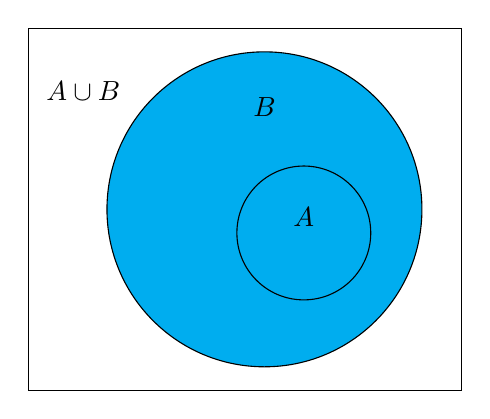
\begin{tikzpicture}
    \draw (-3,-2.3) rectangle (2.5,2.3);
    \draw[fill=cyan] (0,0) circle (2);
    \draw (0.5,-0.3) circle (0.85);
    \node at (0.5,-0.1) {$A$};
    \node at (0,1.3) {$B$};
    \node at (-2.3,1.5) {$A\cup{B}$};
\end{tikzpicture}
            \caption{Figure for Thm.~\ref{thm:Union_With_Subset}}
            \label{fig:Thm_Union_with_Subset}
        \end{figure}
        \begin{theorem}
            \label{thm:Union_of_Subsets_is_Still_Subset}%
            If $A$, $B$, and $C$ are sets, if $A\subseteq{C}$, and if
            $B\subseteq{C}$, then $A\cup{B}\subseteq{C}$.
        \end{theorem}
        \begin{proof}
            For if $B\subseteq{C}$, then $A\cup{B}\subseteq{A}\cup{C}$
            (Thm.~\ref{thm:Union_With_Lesser_Set_on_Right}). But if
            $A\subseteq{C}$, then $A\cup{C}={C}$
            (Thm.~\ref{thm:Union_With_Subset}). And if
            $A\cup{B}\subseteq{A}\cup{C}$ and $A\cup{C}=C$, then
            $A\cup{B}\subseteq{C}$ (Thm.~\ref{thm:Subsets_of_Equal_Sets}).
        \end{proof}
        The converse of Thm.~\ref{thm:Union_With_Subset} can be proved as well.
        \begin{theorem}
            \label{thm:Conv_Union_Is_Bigger}%
            If $A$ and $B$ are sets, and if $A\cup{B}\subseteq{A}$, then
            $A\cup{B}=A$.
        \end{theorem}
        \begin{proof}
            For $A\subseteq{A}\cup{B}$ (Thm.~\ref{thm:Union_is_Bigger_Left}).
            But by hypothesis, $A\cup{B}\subseteq{A}$. But then $A=A\cup{B}$
            (Def.~\ref{def:Equal_Sets}).
        \end{proof}
        \begin{theorem}
            \label{thm:Union_is_Equal}%
            If $A$ and $B$ are sets, and if $A\cup{B}\subseteq{A}$, then
            $B\subseteq{A}$.
        \end{theorem}
        \begin{proof}
            For if $A\cup{B}\subseteq{A}$, then $A\cup{B}=A$
            (Thm.~\ref{thm:Conv_Union_Is_Bigger}). And also,
            $B\subseteq{A}\cup{B}$ (Thm.~\ref{thm:Union_is_Bigger_Right}). But
            if $A\cup{B}=A$ and $B\subseteq{A}\cup{B}$, then $B\subseteq{A}$
            (Thm.~\ref{thm:Subsets_of_Equal_Sets}).
        \end{proof}
        We now prove our claim that the empty set is the only set that acts as a
        zero for \textit{every} set one can name.
        \begin{ltheorem}{Identity Law of Unions}{Identity_Law_of_Unions}
            If $A$ is a set, then $A=\emptyset\cup{A}$ and $A=A\cup\emptyset$.
            \index{Identity Law!of Unions}
        \end{ltheorem}
        \begin{proof}
            For $\emptyset\subseteq{A}$ (Thm.~\ref{thm:Emptyset_Is_Subset}) and
            therefore $\emptyset\cup{A}=A$ (Thm.~\ref{thm:Union_With_Subset}).
            By the commutative law (Thm.~\ref{thm:Commutative_Law_of_Unions}),
            $\emptyset\cup{A}=A\cup\emptyset$ and thus by the transitivity of
            equatility, $A=A\cup\emptyset$
            (Thm.~\ref{thm:Transitivity_of_Equality}).
        \end{proof}
        \begin{theorem}
            \label{thm:Empty_Set_Is_Zero_for_Unions}%
            If $A$ is a set such that, for any set $B$ it is true that
            $A\cup{B}=B$, then $A$ is the empty set.
        \end{theorem}
        \begin{proof}
            For suppose not. If $A\ne\emptyset$, then there is an $x\in{A}$
            (Def.~\ref{def:Empty_Set}). But if $A$ is a set, then $B=\{A\}$ is a
            set (Thm.~\ref{thm:Existence_of_Set_Containing_Set}). But then
            $x\in{A}\cup{B}$ (Def.~\ref{def:Union_of_Two_Sets}). But if
            $x\in{A}$ then $x\ne{A}$
            (Thm.~\ref{thm:Containment_NEqual_Underlying_Set}), and thus
            $x\notin{B}$. But then $A\cup{B}\ne{B}$ (Def.~\ref{def:Equal_Sets}),
            contradicting our hypothesis. Thus, $A$ is the empty set.
        \end{proof}
        \begin{ltheorem}{Idempotent Law of Unions}{Idempotent_Law_of_Unions}
            If $A$ is a set, then $A\cup{A}=A$.
            \index{Idempotent Law!of Unions}
        \end{ltheorem}
        \begin{proof}
            For $A\subseteq{A}$ (Thm.~\ref{thm:Reflexivity_of_Inclusion}) and
            thus $A\cup{A}=A$ (Thm.~\ref{thm:Union_With_Subset}).
        \end{proof}
        Logically, and pedagogically, it would seem appropriate to demonstrate
        the fact that union is an \textit{associative} operation on sets. We
        will do this at the risk of being repetitive since similar results were
        proved for connectives in Chapt.~\ref{chapt:Propositional_Logic}, and
        will again be proven in the more general setting of a Boolean Algebra
        (see \S~\ref{sec:Boolean_Algebra})). Boolean algebras consist of two
        operations that are commutative, distributive, contain identities and
        complements. For the case of sets we will use union and intersection as
        our operations, and the power set of some given set as the set which
        these operations act on. Any system satisfying these properties can then
        prove that the associative law is true for both operations. For the sake
        of completeness, we present the classic arguments that unions and
        intersections are associative, and save the algebraic proofs for the
        more general setting later.
        \begin{theorem}
            \label{thm:Union_with_Equal_Sets}%
            If $A$, $B$, and $C$ are sets, and if $A=B$, then
            $A\cup{C}=B\cup{C}$.
        \end{theorem}
        \begin{proof}
            For if $A=B$, then $A\subseteq{B}$ (Def.~\ref{def:Equal_Sets}). But
            if $A\subseteq{B}$, then $A\cup{C}\subseteq{B}\cup{C}$
            (Thm.~\ref{thm:Union_With_Lesser_Set_on_Left}). But if $A=B$, then
            $B\subseteq{A}$ (Def.~\ref{def:Equal_Sets}), and therefore
            $B\cup{C}\subseteq{A}\cup{C}$
            (Thm.~\ref{thm:Union_With_Lesser_Set_on_Left}), and therefore
            $A\cup{C}=B\cup{C}$ (Def.~\ref{def:Equal_Sets}).
        \end{proof}
        \begin{theorem}
            \label{thm:Lemma_1_for_Assoc_Law_of_Unions}%
            If $A$, $B$, and $C$ are sets, and if $B\subseteq{A}$, then
            $A\cup(B\cup{C})=A\cup{C}$.
        \end{theorem}
        \begin{proof}
            For since $C\subseteq{B}\cup{C}$
            (Thm.~\ref{thm:Union_is_Bigger_Right}), we have that
            $A\cup{C}\subseteq{A}\cup(B\cup{C})$
            (Thm.~\ref{thm:Union_With_Lesser_Set_on_Right}). But since
            $B\subseteq{A}$, it is true that $B\cup{C}\subseteq{A}\cup{C}$
            (Thm.~\ref{thm:Union_With_Lesser_Set_on_Left}). But then
            $A\cup(B\cup{C})\subseteq{A}\cup(A\cup{C})$
            (Thm.~\ref{thm:Union_With_Lesser_Set_on_Right}). But
            $A\subseteq{A}\cup{C}$ (Thm.~\ref{thm:Union_is_Bigger_Left}), and
            thus $A\cup(A\cup{C})=A\cup{C}$ (Thm.~\ref{thm:Union_With_Subset}).
            But if $A\cup(B\cup{C})\subseteq{A}\cup(A\cup{C})$ and
            $A\cup(A\cup{C})=A\cup{C}$, then
            $A\cup(A\cup{B})\subseteq{A}\cup{C}$
            (Thm.~\ref{thm:Subsets_of_Equal_Sets}). But it was proved that
            $A\cup{C}\subseteq{A}\cup(B\cup{C})$, and thus
            $A\cup{C}=A\cup(B\cup{C})$ (Def.~\ref{def:Equal_Sets}).
        \end{proof}
        \begin{theorem}
            \label{thm:Lemma_2_for_Assoc_Law_of_Unions}%
            If $A$, $B$, and $C$ are sets, if $B\subseteq{C}$, then
            $(A\cup{B})\cup{C}=A\cup{C}$.
        \end{theorem}
        \begin{proof}
            For by the commutative law of unions,
            $A\cup{B}=B\cup{A}$. But if $A\cup{B}=B\cup{A}$, then
            $(A\cup{B})\cup{C}=(B\cup{A})\cup{C}$
            (Thm.~\ref{thm:Union_with_Equal_Sets}). But again by the commutative
            law, $(B\cup{A})\cup{C}=C\cup(B\cup{A})$
            (Thm.~\ref{thm:Commutative_Law_of_Unions}). But if
            $B\subseteq{C}$, then $C\cup(B\cup{A})=C\cup{A}$
            (Thm.~\ref{thm:Lemma_1_for_Assoc_Law_of_Unions}). But
            $C\cup{A}=A\cup{C}$ (Thm.~\ref{thm:Commutative_Law_of_Unions}),
            and thus by the transitivity of equality,
            $(A\cup{B})\cup{C}=A\cup{C}$
            (Thm.~\ref{thm:Transitivity_of_Equality}).
        \end{proof}
        With this set of rather trivial results, we can now quickly prove the
        associative law of unions.
        \begin{ltheorem}{Associative Law of Unions}{Associative_Law_of_Unions}
            If $A$, $B$, and $C$ are sets, then
            $A\cup(B\cup{C})=(A\cup{B})\cup{C}$.
            \index{Associative Law!of Unions}
        \end{ltheorem}
        \begin{proof}
            For since $B\subseteq{A}\cup{B}$
            (Thm.~\ref{thm:Union_is_Bigger_Right}), by
            Thm.~\ref{thm:Lemma_1_for_Assoc_Law_of_Unions} we have:
            \begin{equation}
                (A\cup{B})\cup(B\cup{C})=(A\cup{B})\cup{C}
            \end{equation}
            But since $B\subseteq{B}\cup{C}$
            (Thm.~\ref{thm:Union_is_Bigger_Left}),
            by Thm.~\ref{thm:Lemma_2_for_Assoc_Law_of_Unions} we have:
            \begin{equation}
                (A\cup{B})\cup(B\cup{C})=A\cup(B\cup{C})
            \end{equation}
            Thus, by the transitivity of equality,
            $A\cup(B\cup{C})=(A\cup{B})\cup{C}$
            (Thm.~\ref{thm:Transitivity_of_Equality}).
        \end{proof}
        There is a notion called the \textit{principle of duality}%
        \index{Principle of Duality} that applies to unions and intersections.
        Notably, any theorem that applies to unions also applies to
        intersections if we appropriately rearrange the symbols $\subseteq$,
        $\emptyset$, and whatever universe set $U$ we are currently considering.
        In a given proposition we can take the universe to be the union of all
        of the sets hypothesized to exist in the statement of the theorem. This
        duality is made explicit by the distribute laws of unions and
        intersections, as well as the DeMorgan Laws\index{DeMorgan's Laws}.
        \begin{ltheorem}{Commutative Law of Intersections}
                        {Commutative_Law_of_Intersections}
            If $A$ and $B$ are sets, then $A\cap{B}=B\cap{A}$.
            \index{Commutative Law!of Intersections}
        \end{ltheorem}
        \begin{proof}
            For if $x\in{A}\cap{B}$, then $x\in{A}$ and $x\in{B}$
            (Def.~\ref{def:Intersection_of_Two_Sets}). But then $x\in{B}$ and
            $x\in{A}$, and therefore $x\in{B}\cap{A}$
            (Def.~\ref{def:Intersection_of_Two_Sets}). But then for all
            $x\in{A}\cap{B}$ it is true that $x\in{B}\cap{A}$, and therefore
            $A\cup{B}\subseteq{B}\cup{A}$ (Def.~\ref{def:Subsets}). Similarly,
            $B\cap{A}\subseteq{A}\cap{B}$, and thus $A\cap{B}=B\cap{A}$
            (Def.~\ref{def:Equal_Sets}).
        \end{proof}
        \begin{theorem}
            \label{thm:Intersection_is_Smaller_Left}%
            If $A$ snd $B$ are sets, then $A\cap{B}\subseteq{A}$.
        \end{theorem}
        \begin{proof}
            If $x\in{A}\cap{B}$, then $x\in{A}$ and $x\in{B}$
            (Def.~\ref{def:Intersection_of_Two_Sets}), and thus $x\in{A}$.
        \end{proof}
        \begin{theorem}
            \label{thm:Intersection_is_Smaller_Right}%
            If $A$ and $B$ are sets, then $A\cap{B}\subseteq{B}$.
        \end{theorem}
        \begin{proof}
            For $A\cap{B}=B\cap{A}$
            (Thm.~\ref{thm:Commutative_Law_of_Intersections}) and
            $B\cap{A}\subseteq{B}$
            (Thm.~\ref{thm:Intersection_is_Smaller_Left}). But if
            $B\cap{A}\subseteq{B}$ and $B\cap{A}=A\cap{B}$, then
            $A\cap{B}\subseteq{B}$ (Thm.~\ref{thm:Superset_of_Equal_Sets}).
        \end{proof}
        \begin{theorem}
            \label{thm:Intersection_with_Lesser_on_Right}%
            If $A$, $B$, and $C$ are sets, and if $B\subseteq{C}$, then
            $A\cap{B}\subseteq{A}\cap{C}$.
        \end{theorem}
        \begin{proof}
            For if $x\in{A}\cap{B}$, then $x\in{A}$ and $x\in{B}$
            (Def.~\ref{def:Intersection_of_Two_Sets}). But $B$ is a subset of
            $C$ and thus if $x\in{B}$, then $x\in{C}$ (Def.~\ref{def:Subsets}).
            But then $x\in{A}$ and $x\in{C}$, and therefore $x\in{A}\cap{C}$
            (Def.~\ref{def:Intersection_of_Two_Sets}). But
            then $A\cap{B}\subseteq{A}\cap{C}$ (Def.~\ref{def:Subsets}).
        \end{proof}
        \begin{theorem}
            \label{thm:Intersection_with_Lesser_on_Left}%
            If $A$, $B$, and $C$ are sets, and if $B\subseteq{C}$, then
            $B\cap{A}\subseteq{C}\cap{A}$.
        \end{theorem}
        \begin{proof}
            For $B\cap{A}=A\cap{B}$
            (Thm.~\ref{thm:Commutative_Law_of_Intersections}). But if
            $B\subseteq{C}$, then $A\cap{B}\subseteq{A}\cap{C}$
            (Thm.~\ref{thm:Intersection_with_Lesser_on_Right}). But if
            $B\cap{A}=A\cap{B}$ and $A\cap{B}\subseteq{A}\cap{C}$, then
            $B\cap{A}\subseteq{A}\cap{C}$
            (Thm.~\ref{thm:Superset_of_Equal_Sets}). But $A\cap{C}=C\cap{A}$
            (Thm.~\ref{thm:Commutative_Law_of_Intersections}), and if
            $B\cap{A}\subseteq{A}\cap{C}$ and $A\cap{C}=C\cap{A}$, then
            $B\cap{A}\subseteq{C}\cap{A}$
            (Thm.~\ref{thm:Subsets_of_Equal_Sets}).
        \end{proof}
        \begin{theorem}
            \label{thm:A_cap_B_Subset_C_cap_D}%
            If $A$, $B$, $C$, and $D$ are sets, if $A\subseteq{C}$, and if
            $B\subseteq{D}$, then $A\cap{B}\subseteq{C}\cap{D}$.
        \end{theorem}
        \begin{proof}
            For if $B\subseteq{D}$, then $A\cap{B}\subseteq{A}\cap{D}$
            (Thm.~\ref{thm:Intersection_with_Lesser_on_Right}). But if
            $A\subseteq{C}$, then $A\cap{D}\subseteq{C}\cap{D}$
            (Thm.~\ref{thm:Intersection_with_Lesser_on_Left}). But if
            $A\cap{B}\subseteq{A}\cap{D}$ and $A\cap{D}\subseteq{C}\cap{D}$,
            then $A\cap{B}\subseteq{C}\cap{D}$
            (Thm.~\ref{thm:Transitivity_of_Inclusion}).
        \end{proof}
        \begin{theorem}
            \label{thm:Intersection_with_Subset}%
            If $A$ and $B$ are sets, and if $A\subseteq{B}$, then $A\cap{B}=A$.
        \end{theorem}
        \begin{proof}
            For $A\cap{B}\subseteq{A}$
            (Thm.~\ref{thm:Intersection_is_Smaller_Left}). But if
            $A\subseteq{B}$, then for all $x\in{A}$ it is true that $x\in{B}$
            (Def.~\ref{def:Subsets}). Thus if $x\in{A}$, then $x\in{A}$ and
            $x\in{B}$, and therefore $x\in{A}\cap{B}$
            (Def.~\ref{def:Intersection_of_Two_Sets}), hence
            $A\subseteq{A}\cap{B}$. Thus, $A=A\cap{B}$
            (Def.~\ref{def:Equal_Sets}).
        \end{proof}
        \begin{figure}[H]
            \centering
            \captionsetup{type=figure}
            \centering
            \documentclass[crop,class=article]{standalone}
%----------------------------Preamble-------------------------------%
\usepackage{tikz}                       % Drawing/graphing tools.
%--------------------------Main Document----------------------------%
\begin{document}
    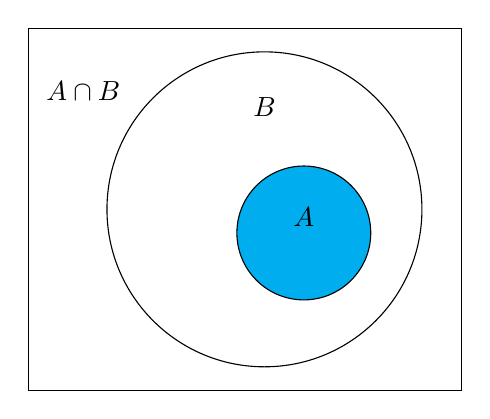
\begin{tikzpicture}
        \draw (-3,-2.3) rectangle (2.5,2.3);
        \draw (0,0) circle (2);
        \draw[fill=cyan] (0.5,-0.3) circle (0.85);
        \node at (0.5,-0.1) {$A$};
        \node at (0,1.3) {$B$};
        \node at (-2.3,1.5) {$A\cap{B}$};
    \end{tikzpicture}
\end{document}
            \caption{Visual for Thm.~\ref{thm:Intersection_with_Subset}.}
            \label{fig:Intersection_with_Subset}
        \end{figure}
        \begin{theorem}
            \label{thm:A_sub_B_sub_C_and_A_cap_C_eq_B}%
            If $A$, $B$, and $C$ are sets, if $A\subseteq{B}$, if
            $B\subseteq{C}$, and if $A\cap{C}=B$, then $A=B$.
        \end{theorem}
        \begin{proof}
            For if $A\subseteq{B}$ and $B\subseteq{C}$, then $A\subseteq{C}$
            (Thm.~\ref{thm:Transitivity_of_Inclusion}). But if $A\subseteq{C}$,
            then $A\cap{C}=A$ (Thm.~\ref{thm:Intersection_with_Subset}). But
            $A\cap{C}=B$, and therefore $A=B$
            (Thm.~\ref{thm:Transitivity_of_Equality}).
        \end{proof}
        \begin{theorem}
            \label{thm:Intersection_of_Supersets_is_Still_Superset}%
            If $A$, $B$, and $C$ are sets, if $A\subseteq{B}$, and if
            $A\subseteq{C}$, then $A\subseteq{B}\cap{C}$.
        \end{theorem}
        \begin{proof}
            For if $A\subseteq{B}$, then $A\cap{C}\subseteq{B}\cap{C}$
            (Thm.~\ref{thm:Intersection_with_Lesser_on_Left}). But if
            $A\subseteq{C}$, then $A\cap{C}=A$
            (Thm.~\ref{thm:Intersection_with_Subset}). But if $A=A\cap{C}$
            and $A\cap{C}\subseteq{B}\cap{C}$, then $A\subseteq{A}\cap{C}$
            (Thm.~\ref{thm:Superset_of_Equal_Sets}).
        \end{proof}
        \begin{theorem}
            \label{thm:Conv_Intersection_with_Subset}%
            If $A$ and $B$ are sets, and if $A\subseteq{A}\cap{B}$, then
            $A=A\cap{B}$.
        \end{theorem}
        \begin{proof}
            For $A\cap{B}\subseteq{A}$
            (Thm.~\ref{thm:Intersection_is_Smaller_Left}). But by hypothesis,
            $A\subseteq{A}\cap{B}$, and thus $A=A\cap{B}$
            (Def.~\ref{def:Equal_Sets}).
        \end{proof}
        \begin{theorem}
            \label{thm:Intersection_is_Equal}%
            If $A$ and $B$ are sets, and if $A=A\cap{B}$, then $A\subseteq{B}$.
        \end{theorem}
        \begin{proof}
            For if $A=A\cap{B}$, then $A\subseteq{A}\cap{B}$
            (Def.~\ref{def:Equal_Sets}). But $A\cap{B}\subseteq{B}$
            (Thm.~\ref{thm:Intersection_is_Smaller_Right}) and thus by the
            transitivity of inclusion, $A\subseteq{B}$
            (Thm.~\ref{thm:Transitivity_of_Inclusion}).
        \end{proof}
        In Thm.~\ref{thm:Identity_Law_of_Unions} we proved that the empty set is
        an identity for unions. That is, for any set $A$ it is true that
        $A=\emptyset\cup{A}$ and $A=A\cup\emptyset$. There is no legal identity
        law of intersections\index{Identity Law!of Intersections}. We proved
        that for any two sets $A$ and $B$ such that $A\subseteq{B}$, it is then
        true that $A\cap{B}=A$. If there were some \textit{universe set} $U$,
        then $A\cap{U}=A$ and thus $U$ acts as the identity of intersections. In
        many contexts there is such a universe, notably the power set of some
        given set that is of current consideration, but there is no general
        universe set since this amounts to a set of all sets, which we've proved
        is impossible under the axioms of ZFC.
        \begin{theorem}
            \label{thm:Intersection_with_Emptyset}%
            If $A$ is a set, then $\emptyset\cap{A}=\emptyset$.
        \end{theorem}
        \begin{proof}
            For $\emptyset\subseteq{A}$ (Thm.~\ref{thm:Emptyset_Is_Subset}), and
            therefore $\emptyset\cap{A}=\emptyset$
            (Thm.~\ref{thm:Intersection_with_Subset}).
        \end{proof}
        \begin{theorem}
            \label{thm:Empty_Set_Is_Zero_for_Intersections}%
            If $A$ is a set such that for any set $B$ it is true that
            $A\cap{B}=A$, then $A=\emptyset$.
        \end{theorem}
        \begin{proof}
            For $A\cap\emptyset=\emptyset\cap{A}$
            (Thm.~\ref{thm:Commutative_Law_of_Intersections}) and
            $\emptyset\cap{A}=\emptyset$
            (Thm.~\ref{thm:Intersection_with_Emptyset}). Thus, by the
            transitivity of equality, $A\cap\emptyset=\emptyset$
            (Thm.~\ref{thm:Transitivity_of_Equality}). But by hypothesis,
            $A\cap\emptyset=A$. Again by transitivity, $A=\emptyset$
            (Thm.~\ref{thm:Transitivity_of_Equality}).
        \end{proof}
        \begin{ltheorem}{Idempotent Law of Intersections}
                        {Idempotent_Law_of_Intersections}
            If $A$ is a set, then $A\cap{A}=A$.
            \index{Idempotent Law!of Intersections}
        \end{ltheorem}
        \begin{proof}
            For $A\subseteq{A}$ (Thm.~\ref{thm:Reflexivity_of_Inclusion}) and
            thus $A\cap{A}=A$ (Thm.~\ref{thm:Intersection_with_Subset}).
        \end{proof}
        \begin{theorem}
            \label{thm:Intersection_of_Subsets_is_Still_Subset}%
            If $A$, $B$, and $C$ are sets, if $A\subseteq{C}$, and if
            $B\subseteq{C}$, then $A\cap{B}\subseteq{C}$.
        \end{theorem}
        \begin{proof}
            For if $A\subseteq{C}$ and $B\subseteq{C}$, then
            $A\cap{B}\subseteq{C}\cap{C}$
            (Thm.~\ref{thm:A_cap_B_Subset_C_cap_D}). But $C\cap{C}=C$
            (Thm.~\ref{thm:Idempotent_Law_of_Intersections}). But if
            $A\cap{B}\subseteq{C}\cap{C}$ and $C\cap{C}=C$, then
            $A\cap{B}\subseteq{C}$ (Thm.~\ref{thm:Subsets_of_Equal_Sets}).
        \end{proof}
        \begin{theorem}
            \label{thm:Intersection_with_Equal_Sets}%
            If $A$, $B$, and $C$ are sets, and if $B=C$, then
            $A\cap{B}=A\cap{C}$.
        \end{theorem}
        \begin{proof}
            For if $B=C$, then $B\subseteq{C}$ (Def.~\ref{def:Equal_Sets}).
            But if $B\subseteq{C}$, then $A\cap{B}\subseteq{A}\cap{C}$
            (Thm.~\ref{thm:Intersection_with_Lesser_on_Right}). But if $B=C$,
            then $C\subseteq{B}$ (Def.~\ref{def:Equal_Sets}). But if
            $C\subseteq{B}$, then $A\cap{C}\subseteq{A}\cap{B}$
            (Thm.~\ref{thm:Intersection_with_Lesser_on_Right}). But it was just
            proved that $A\cap{B}\subseteq{A}\cap{C}$, and thus
            $A\cap{B}=A\cap{C}$ (Def.~\ref{def:Equal_Sets}).
        \end{proof}
        \begin{theorem}
            \label{thm:Lemma_1_for_Assoc_Law_of_Intersections}%
            If $A$, $B$, and $C$ are sets, and if $A\subseteq{B}$, then
            $A\cap(B\cap{C})=A\cap{C}$.
        \end{theorem}
        \begin{proof}
            For since $B\cap{C}\subseteq{C}$
            (Thm.~\ref{thm:Intersection_is_Smaller_Right}) it is true that
            $A\cap(B\cap{C})\subseteq{A}\cap{C}$
            (Thm.~\ref{thm:Intersection_with_Lesser_on_Right}). But since
            $A\subseteq{B}$ it is true that $A\cap{C}\subseteq{B}\cap{C}$
            (Thm.~\ref{thm:Intersection_with_Lesser_on_Left}). But then
            $A\cap(A\cap{C})\subseteq{A}\cap(B\cap{C})$
            (Thm.~\ref{thm:Intersection_with_Lesser_on_Right}). But
            $A\cap{C}\subseteq{A}$ (Thm.~\ref{thm:Intersection_is_Smaller_Left})
            and thus $A\cap(A\cap{C})=A\cap{C}$
            (Thm.~\ref{thm:Intersection_with_Subset}). But if
            $A\cap{C}=A\cap(A\cap{C})$ and
            $A\cap(A\cap{C})\subseteq{A}\cap(B\cap{C})$, then
            $A\cap{C}\subseteq{A}\cap(B\cap{C})$
            (Thm.~\ref{thm:Superset_of_Equal_Sets}). Thus,
            $A\cap(B\cap{C})=A\cap{C}$ (Def.~\ref{def:Equal_Sets}).
        \end{proof}
        \begin{theorem}
            \label{thm:Lemma_2_for_Assoc_Law_of_Intersections}%
            If $A$, $B$, and $C$ are sets, and if $C\subseteq{B}$, then
            $(A\cap{B})\cap{C}=A\cap{C}$.
        \end{theorem}
        \begin{proof}
            For $A\cap{B}=B\cap{A}$
            (Thm.~\ref{thm:Commutative_Law_of_Intersections}), and thus
            $(A\cap{B})\cap{C}=(B\cap{A})\cap{C}$
            (Thm.~\ref{thm:Intersection_with_Equal_Sets}). But
            $(B\cap{A})\cap{C}=C\cap(B\cap{A})$
            (Thm.~\ref{thm:Commutative_Law_of_Intersections}). But if
            $C\subseteq{B}$, then $C\cap(B\cap{A})=C\cap{A}$
            (Thm.~\ref{thm:Lemma_1_for_Assoc_Law_of_Intersections}). But
            $C\cap{A}=A\cap{C}$
            (Thm.~\ref{thm:Commutative_Law_of_Intersections}), and thus by
            transitivity, $(A\cap{B})\cap{C}=A\cap{C}$
            (Thm.~\ref{thm:Transitivity_of_Equality}).
        \end{proof}
        And now we completely mimic the proof of the associative law of unions,
        and derive the associativity of intersections.
        \begin{ltheorem}{Associative Law of Intersections}
                        {Associative_Law_of_Intersections}
            If $A$, $B$, and $C$ are sets, then
            $A\cap(B\cap{C})=(A\cap{B})\cap{C}$.
            \index{Associative Law!of Intersections}
        \end{ltheorem}
        \begin{proof}
            For since $A\cap{B}\subseteq{B}$
            (Thm.~\ref{thm:Intersection_is_Smaller_Right}), by
            Thm.~\ref{thm:Lemma_1_for_Assoc_Law_of_Intersections} we have:
            \begin{equation}
                (A\cap{B})\cap(B\cap{C})=(A\cap{B})\cap{C}
            \end{equation}
            But since $B\cap{C}\subseteq{B}$
            (Thm.~\ref{thm:Intersection_is_Smaller_Left}),
            by Thm.~\ref{thm:Lemma_2_for_Assoc_Law_of_Intersections} we have:
            \begin{equation}
                (A\cap{B})\cap(B\cap{C})=A\cap(B\cap{C})
            \end{equation}
            Thus, by the transitivity of equality,
            $A\cap(B\cap{C})=(A\cap{B})\cap{C}$
            (Thm.~\ref{thm:Transitivity_of_Equality}).
        \end{proof}
        We now move on to the distributive laws of unions and intersections.
        Thus far the theorems proved have dealt solely with unions or with
        intersections, but have not mixed the two. Associativity nows tells us
        that an expression of the form $A\cup{B}\cup{C}$ is no longer
        ambiguous since $A\cup(B\cup{C})=(A\cup{B})\cup{C}$, and thus we may rid
        ourselves of the burden of writing parantheses. Similarly,
        $A\cap{B}\cap{C}$ is well-defined now. There is still an air of mystery
        surrounding an expression such as $A\cap{B}\cup{C}$. Should this mean
        $A\cap(B\cup{C})$ or $(A\cap{B})\cup{C}$, and are these equal? The
        distributive laws tell us how to simplify such a thing, but
        unfortunately these theorems tell us that parantheses are essential for
        when mixing intersections and unions. That is, as we will see, an
        expression of the form $A\cap{B}\cup{C}$ is indeed undefined without
        the introduction of parantheses: $A\cap(B\cup{C})$ need not be equal to
        $(A\cap{B})\cup{C}$.
        \begin{theorem}
            \label{thm:First_Pseudo_Dist_Law_Union}%
            If $A$, $B$, and $C$ are sets, then
            $B\cap{C}\subseteq(A\cup{B})\cap(A\cup{C})$.
        \end{theorem}
        \begin{proof}
            For by Thm.~\ref{thm:Union_is_Bigger_Right} we have that
            $B\subseteq{A}\cup{B}$ and $C\subseteq{A}\cup{C}$, and therefore
            $B\cap{C}\subseteq(A\cup{C})\cap(A\cup{C})$
            (Thm.~\ref{thm:A_cap_B_Subset_C_cap_D}).
        \end{proof}
        \begin{theorem}
            \label{thm:Second_Pseudo_Dist_Law_Union}%
            If $A$, $B$, and $C$ are sets, then
            $A\cup(B\cap{C})\subseteq(A\cup{B})\cap(A\cup{C})$.
        \end{theorem}
        \begin{proof}
            For $A\subseteq{A}\cup{B}$ and $A\subseteq{A}\cup{C}$
            (Thm.~\ref{thm:Union_is_Bigger_Left}), and therefore it is true that
            $A\cap{A}\subseteq(A\cup{B})\cap(A\cup{C})$
            (Thm.~\ref{thm:A_cup_B_Subset_C_cup_D}). But $A=A\cap{A}$
            (Thm.~\ref{thm:Idempotent_Law_of_Unions}), and if
            $A=A\cap{A}$ and $A\cap{A}\subseteq(A\cup{B})\cap(A\cup{C})$, then
            $A\subseteq(A\cup{B})\cap(A\cup{C})$
            (Thm.~\ref{thm:Superset_of_Equal_Sets}). But
            $B\cap{C}\subseteq(A\cup{B})\cap(A\cup{C})$
            (Thm.~\ref{thm:First_Pseudo_Dist_Law_Union}), and therefore:
            \begin{equation}
                A\cap(B\cup{C})\subseteq
                \big((A\cup{B})\cap(A\cup{C})\big)\cap
                \big((A\cup{B})\cap(A\cup{C})\big)
                =(A\cup{B})\cap(A\cup{C})
            \end{equation}
            Where this last equality is by the idempotent law of intersections
            (Thm.~\ref{thm:Idempotent_Law_of_Intersections}). But then
            $A\cap(B\cup{C})\subseteq(A\cup{B})\cap(A\cup{C})$
            (Thm.~\ref{thm:Subsets_of_Equal_Sets}).
        \end{proof}
        This proves half of the distributive law of unions which states that
        $A\cup(B\cap{C})=(A\cup{B})\cap(A\cup{C})$. That is, unions distribute
        over intersections. To prove the opposite direction of this equality
        seems to resist algebraic efforts and one must rely directly on the use
        of the containment symbol (\gls{containmentsymb}). However, once one has
        one of the distributive laws, the latter may be proved with purely
        algebraic arguments. We will do so presently.
        \newpage
        \begin{ftheorem}{Distributive Law of Unions}{Distributive_Law_of_Unions}
            If $A$, $B$, and $C$ are sets, then:
            \begin{equation*}
                A\cup(B\cap{C})=(A\cup{B})\cap(A\cup{C})
            \end{equation*}
        \end{ftheorem}
        \begin{bproof}
            For suppose not. But
            $A\cup(B\cap{C})\subseteq(A\cup{B})\cap(A\cup{C})$
            (Thm.~\ref{thm:Second_Pseudo_Dist_Law_Union}), and therefore
            $A\cup(B\cap{C})\subsetneq(A\cup{B})\cap(A\cup{C})$
            (Def.~\ref{def:Proper_Subsets}). But then there is an
            $x\in(A\cup{B})\cap(A\cup{C})$ such that $x\notin{A}\cup(B\cap{C})$
            (Thm.~\ref{thm:Prop_Subset_Not_Equal}). But if
            $x\notin{A}\cup(B\cap{C})$, then $x\notin{A}$ and
            $x\notin{B}\cap{C}$ (Def.~\ref{def:Union_of_Two_Sets}). But
            $x\in(A\cup{B})\cap(A\cup{C})$, and therefore $x\in{A}\cup{B}$ and
            $x\in{A}\cup{C}$ (Def.~\ref{def:Intersection_of_Two_Sets}). But
            $x\notin{A}$, and thus if $x\in{A}\cup{B}$ then it must be true
            that $x\in{B}$. And similarly, since $x\in{A}\cup{C}$, it must be
            true that $x\in{C}$. But then $x\in{B}$ and $x\in{C}$, and therefore
            $x\in{B}\cap{C}$ (Def.~\ref{def:Intersection_of_Two_Sets}), a
            contradiction. This completes the proof.
        \end{bproof}
        We can visualize Thm.~\ref{thm:Distributive_Law_of_Unions} with Venn
        diagrams
        (Fig.~\ref{fig:Venn_Diagram_Distributive_Law_of_Unions}).
        \begin{figure}[H]
            \centering
            \captionsetup{type=figure}
            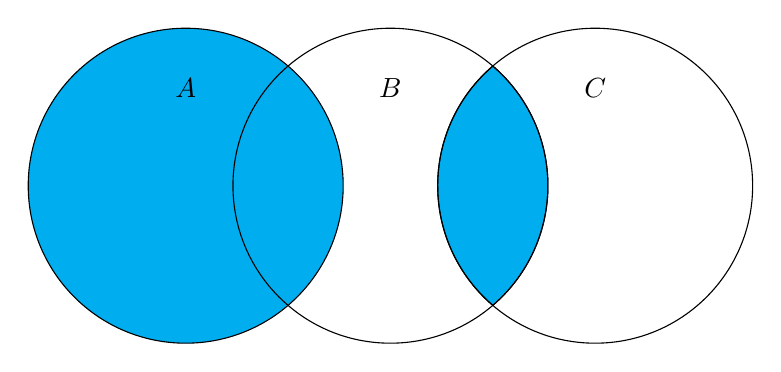
\begin{tikzpicture}
    % Coordinates for the points.
    \coordinate (A) at (-2.6, 0.0);
    \coordinate (B) at ( 0.0, 0.0);
    \coordinate (C) at ( 2.6, 0.0);

    % Fill in the circle A.
    \draw[fill=cyan, draw=none] (A) circle (2);

    % Fill in the overlap between B and C.
    \draw[fill=cyan] (1.3, -1.51987) arc(-49.46:49.46:2) arc(130.54:229.46:2);

    % Draw circles outlining the regions A, B, and C.
    \draw[draw=black] (A) circle (2);
    \draw[draw=black] (B) circle (2);
    \draw[draw=black] (C) circle (2);

    % Add some labels.
    \node at (A) [above=1cm] {$A$};
    \node at (B) [above=1cm] {$B$};
    \node at (C) [above=1cm] {$C$};
\end{tikzpicture}
            \caption{Venn Diagram for Distributive Law of Unions}
            \label{fig:Venn_Diagram_Distributive_Law_of_Unions}
        \end{figure}
        \begin{ftheorem}{Distributive Law of Intersections}
                        {Distributive_Law_of_Intersections}
            If $A$, $B$, and $C$ are sets, then:
            \begin{equation*}
                A\cap(B\cup{C})=(A\cap{B})\cup(A\cap{C})
            \end{equation*}
        \end{ftheorem}
        \begin{bproof}
            For $(A\cap{B})\cup(A\cap{C})=\big((A\cap{B})\cup{A}\big)%
                 \cap\big((A\cap{B})\cup{C}\big)$
            (Thm.~\ref{thm:Distributive_Law_of_Unions}). But
            $A\cap{B}\subseteq{A}$ (Thm.~\ref{thm:Intersection_is_Smaller_Left})
            and therefore $(A\cap{B})\cup{A}=A$
            (Thm.~\ref{thm:Union_With_Subset}). But then
            $\big((A\cap{B})\cup{A}\big)\cap\big((A\cap{B})\cup{C}\big)%
             =A\cap\big((A\cap{B})\cup{C}\big)$
            (Thm.~\ref{thm:Intersection_with_Equal_Sets}). But
            $(A\cap{B})\cup{C}=C\cup(A\cap{B})$
            (Thm.~\ref{thm:Commutative_Law_of_Unions}) and
            $C\cup(A\cap{B})=(C\cup{A})\cap(C\cup{B})$
            (Thm.~\ref{thm:Distributive_Law_of_Unions}). But then
            $A\cap\big((A\cap{B})\cup{C}\big)%
             =A\cap\big((C\cup{A})\cap(C\cup{B})\big)$
            (Thm.~\ref{thm:Intersection_with_Equal_Sets}). But
            $A\cap\big((C\cup{A})\cap(C\cup{B})\big)%
             =\big(A\cap(C\cup{A})\big)\cap(C\cup{B})$
            (Thm.~\ref{thm:Associative_Law_of_Unions}). And since
            $A\subseteq{C}\cup{A}$ (Thm.~\ref{thm:Union_is_Bigger_Right}), we
            have that $A\cap(C\cup{A})=A$
            (Thm.~\ref{thm:Intersection_with_Subset}). But then
            $\big(A\cap(C\cup{A})\big)\cap(C\cup{B})=A\cap(C\cup{B})$
            (Thm.~\ref{thm:Intersection_with_Equal_Sets}). But
            $C\cup{B}=B\cup{C}$ (Thm.~\ref{thm:Commutative_Law_of_Unions}),
            and thus $A\cap(C\cup{B})=A\cap(B\cup{C})$
            (Thm.~\ref{thm:Intersection_with_Equal_Sets}).
            Thus by transitivity, $(A\cap{B})\cup(A\cap{C})=A\cap(B\cup{C})$
            (Thm.~\ref{thm:Transitivity_of_Equality}).
        \end{bproof}
        \begin{figure}[H]
            \centering
            \captionsetup{type=figure}
            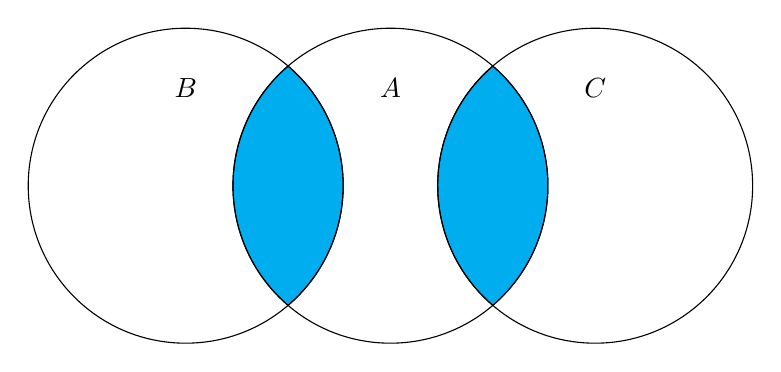
\begin{tikzpicture}
    % Coordinates for the points.
    \coordinate (B) at (-2.6, 0.0);
    \coordinate (A) at ( 0.0, 0.0);
    \coordinate (C) at ( 2.6, 0.0);

    % Fill in the overlap between B and A.
    \draw[fill=cyan] (-1.3, -1.51987) arc(-49.46:49.46:2) arc(130.54:229.46:2);

    % Fill in the overlap between A and C.
    \draw[fill=cyan] (1.3, -1.51987) arc(-49.46:49.46:2) arc(130.54:229.46:2);

    % Draw circles outlining the regions A, B, and C.
    \draw[draw=black] (A) circle (2);
    \draw[draw=black] (B) circle (2);
    \draw[draw=black] (C) circle (2);

    % Add some labels.
    \node at (A) [above=1cm] {$A$};
    \node at (B) [above=1cm] {$B$};
    \node at (C) [above=1cm] {$C$};
\end{tikzpicture}
            \caption{Venn Diagram for the Distributive Law of Intersections}
            \label{fig:Venn_Diagram_Distributive_Law_of_Intersections}
        \end{figure}
        \begin{theorem}
            \label{thm:Dist_Law_Inter_Subset_of_Dist_Law_Union}%
            If $A$, $B$, and $C$ are sets, then
            $A\cap(B\cup{C})\subseteq{A}\cup(B\cap{C})$.
        \end{theorem}
        \begin{proof}
            For $A\cap(B\cup{C})\subseteq{A}$
            (Thm.~\ref{thm:Intersection_is_Smaller_Left}) and
            $A\subseteq{A}\cup(B\cap{C})$ (Thm.~\ref{thm:Union_is_Bigger_Left}),
            and thus $A\cap(B\cup{C})\subseteq{A}\cup(B\cap{C})$
            (Thm.~\ref{thm:Transitivity_of_Inclusion}).
        \end{proof}
        We can use Venn diagrams to visualize this more clearly (see
        Fig.~\ref{fig:Venn_Diagram_Compare_Dist_Laws_Unions_Intersections}).
        \begin{figure}[H]
            \centering
            \captionsetup{type=figure}
            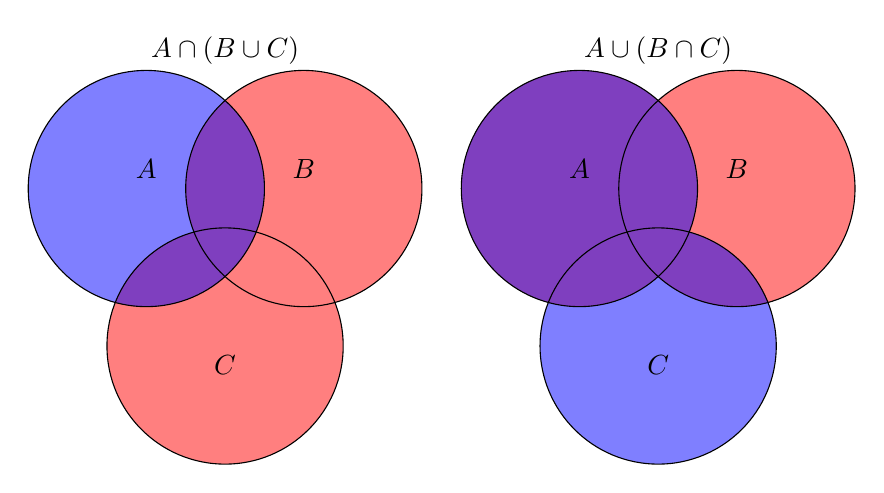
\begin{tikzpicture}[scale=0.5]
    \begin{scope}[xshift=5.5cm]
        \coordinate (A) at (-2,  2);
        \coordinate (B) at ( 2,  2);
        \coordinate (C) at ( 0, -2);

        \begin{scope}
            \clip (A) circle (3cm) (B) circle (3cm);
            \fill[red, opacity=0.5] (-5, -5) rectangle (5, 5);
        \end{scope}

        \begin{scope}
            \clip (A) circle (3cm) (C) circle (3cm);
            \fill[blue, opacity=0.5] (-5, -5) rectangle (5, 5);
        \end{scope}

        \draw (A) circle (3cm);
        \draw (B) circle (3cm);
        \draw (C) circle (3cm);

        \node at (A) [above] {$A$};
        \node at (B) [above] {$B$};
        \node at (C) [below] {$C$};
        \node at (0, 5.5) {$A\cup(B\cap{C})$};
    \end{scope}

    \begin{scope}[xshift=-5.5cm]
        \coordinate (A) at (-2,  2);
        \coordinate (B) at ( 2,  2);
        \coordinate (C) at ( 0, -2);

        \begin{scope}
            \clip (B) circle (3cm) (C) circle (3cm);
            \fill[red, opacity=0.5] (-5, -5) rectangle (5, 5);
        \end{scope}

        \begin{scope}
            \clip (A) circle (3cm);
            \fill[blue, opacity=0.5] (-5, -5) rectangle (5, 5);
        \end{scope}

        \draw (A) circle (3cm);
        \draw (B) circle (3cm);
        \draw (C) circle (3cm);

        \node at (A) [above] {$A$};
        \node at (B) [above] {$B$};
        \node at (C) [below] {$C$};
        \node at (0, 5.5) {$A\cap(B\cup{C})$};
    \end{scope}
\end{tikzpicture}
            \caption{Figure for
                     Thm.~\ref{thm:Dist_Law_Inter_Subset_of_Dist_Law_Union}}
            \label{fig:Venn_Diagram_Compare_Dist_Laws_Unions_Intersections}
        \end{figure}
        We now introduce a new set operation called
        \textit{set difference}\index{Set!Difference}. In many respects this is
        analogous to the operation of subtraction one finds in arithmetic. One
        should be careful since there are many situations in which the analogy
        breaks down.
        \begin{theorem}
            \label{thm:Existence_of_Set_Difference}%
            If $A$ and $B$ are sets, then there is a set $C$ such that for all
            $x$ it is true that $x\in{C}$ if and only if $x\in{A}$ and
            $x\notin{B}$.
        \end{theorem}
        \begin{proof}
            For let $P$ be the proposition \textit{true if} $x\notin{B}$,
            \textit{false otherwise}. Then by the axiom schema of specification
            (Ax.~\ref{ax:Axiom_Schema_of_Specification}), there is a set $C$
            such that:
            \begin{equation}
                C=\{\,x\in{A}\;|\;P(x)\,\}
            \end{equation}
            But then $x\in{C}$ if and only if $x\in{A}$ and $P(x)$ is true.
            But $P(x)$ is true if and only if $x\notin{B}$. Thus $x\in{C}$ if
            and only if $x\in{A}$ and $x\notin{B}$.
        \end{proof}
        The set described in Thm.~\ref{thm:Existence_of_Set_Difference} is known
        as the set difference of $B$ with respect to $A$. We take a moment to
        discuss some of it's properties, as well as the related notion of
        \textit{complement}\index{Complement!of a Set}
        \begin{fdefinition}{Set Difference}{Set_Difference}
            The set difference of a set $B$ with respect to a set $A$ is the
            set:\index{Set Difference}
            \begin{equation*}
                A\setminus{B}=\{\,x\in{A}\;|\;x\notin{B}\,\}
            \end{equation*}
        \end{fdefinition}
        \begin{example}
            Let $\mathbb{Z}$ denote the integers, and $\mathbb{N}$ denote the
            set of natural numbers. Then $\mathbb{Z}\setminus\mathbb{N}$ is the
            set of all negative integers. Flipping this, we see that
            $\mathbb{N}\setminus\mathbb{Z}$ is the empty set since there are no
            non-negative integers that are not also integers.
        \end{example}
        \begin{example}
            Letting $\mathbb{R}$ denote the real numbers and $\mathbb{Q}$ denote
            the rationals, $\mathbb{R}\setminus\mathbb{Q}$ is the set of all
            \textit{irrational} numbers. Famous examples include $\sqrt{2}$,
            $\pi$, and $e$ (sometimes known as Euler's constant).
        \end{example}
        \begin{example}
            If we let $A$ and $B$ be defined as:
            \par
            \begin{subequations}
                \begin{minipage}[b]{0.49\textwidth}
                    \centering
                    \begin{equation}
                        A=\{\,a,\,b,\,c\,\}
                    \end{equation}
                \end{minipage}
                \hfill
                \begin{minipage}[b]{0.49\textwidth}
                    \centering
                    \begin{equation}
                        B=\{\,b,\,c,\,d\,\}
                    \end{equation}
                \end{minipage}
            \end{subequations}
            \par\vspace{2.5ex}
            Then we can compute directly the set difference between the two:
            \par
            \begin{subequations}
                \begin{minipage}[b]{0.49\textwidth}
                    \centering
                    \begin{equation}
                        A\setminus{B}=\{\,a\,\}
                    \end{equation}
                \end{minipage}
                \hfill
                \begin{minipage}[b]{0.49\textwidth}
                    \centering
                    \begin{equation}
                        B\setminus{A}=\{\,d\,\}
                    \end{equation}
                \end{minipage}
            \end{subequations}
            \par\vspace{2.5ex}
            Thus set difference between sets is not a \textit{commutative} set
            operation.
        \end{example}
        Set difference an be visualize, much like unions and intersections, via
        the use of Venn diagrams (Fig.~\ref{fig:Set_Diff_Venn_Diagram}).
        \begin{figure}[H]
            \centering
            \captionsetup{type=figure}
            %--------------------------------Dependencies----------------------------------%
%   tikz                                                                       %
%-------------------------------Main Document----------------------------------%
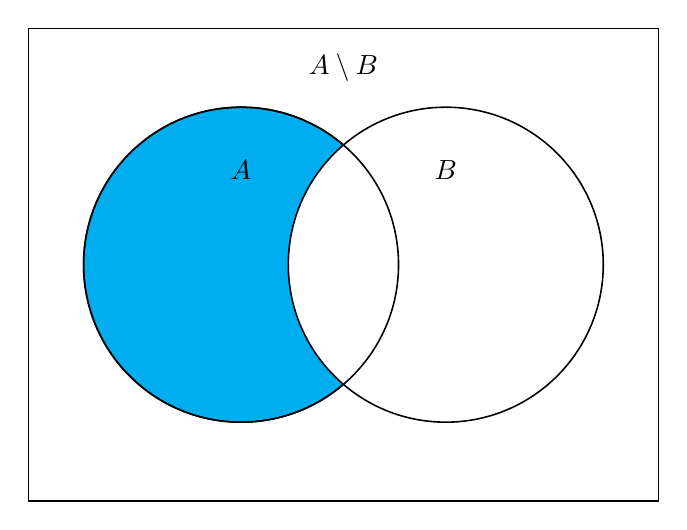
\begin{tikzpicture}[line width=0.2mm]

    % Coordinates for the centers of the circles.
    \coordinate (C1) at (-1.3, 0);
    \coordinate (C2) at ( 1.3, 0);

    % Coordinates for the labels.
    \coordinate (A) at (-1.3, 1.2);
    \coordinate (B) at ( 1.3, 1.2);
    \coordinate (U) at ( 0.0, 2.5);

    % Rectangle indicating the universe set.
    \draw (-4, -3) rectangle (4, 3);

    % Draw the two circles.
    \draw[fill=cyan]              (C1) circle (2);
    \draw[fill=white, draw=black] (C2) circle (2);

    % Add an outline to the left circle.
    \draw (C1) circle (2);

    % Labels.
    \node at (A) {$A$};
    \node at (B) {$B$};
    \node at (U) {$A\setminus{B}$};
\end{tikzpicture}
            \caption{Venn Diagram for Set Difference}
            \label{fig:Set_Diff_Venn_Diagram}
        \end{figure} 
        \begin{theorem}
            \label{thm:Set_Difference_of_Set_with_Self}%
            If $A$ is a set, then $A\setminus{A}=\emptyset$.
        \end{theorem}
        \begin{proof}
            For suppose not. Then there is an $x\in{A}\setminus{A}$
            (Def.~\ref{def:Empty_Set}). But then $x\in{A}$ and $x\notin{A}$
            (Def.~\ref{def:Set_Difference}), a contradiction.
        \end{proof}
        \begin{theorem}
            \label{thm:Set_Difference_is_Subset}%
            If $A$ and $B$ are sets, then $A\setminus{B}\subseteq{A}$.
        \end{theorem}
        \begin{proof}
            For suppose not. Then there is an $x\in{A}\setminus{B}$ such that
            $x\notin{A}$. But $x\in{A}\setminus{B}$ if and only if $x\in{A}$ and
            $x\notin{B}$ (Def.~\ref{def:Set_Difference}), and thus $x\in{A}$, a
            contradiction.
        \end{proof}
        \begin{theorem}
            \label{thm:Set_Difference_of_Set_and_Empty}%
            If $A$ is a set, then $A\setminus\emptyset=A$.
        \end{theorem}
        \begin{proof}
            For suppose not. Since $A\setminus\emptyset\subseteq{A}$
            (Thm.~\ref{thm:Set_Difference_is_Subset}), there is an $x\in{A}$
            such that $x\notin{A}\setminus\emptyset$
            (Def.~\ref{def:Equal_Sets}). But if $x\in{A}$ and
            $x\notin{A}\setminus\emptyset$, then $x\in\emptyset$
            (Def.~\ref{def:Set_Difference}) a contradiction since
            $x\notin\emptyset$ (Def.~\ref{def:Empty_Set}).
        \end{proof}
        While set difference appears similar to subtraction, the two have their
        differences. For any two real numbers $a$ and $b$, it is always true
        that $b=a-(a-b)$. For sets this is not true. For let $A$ be the empty
        set, and let $B$ be non-empty. Then
        $A\setminus(A\setminus{B})=\emptyset$, which is not $B$. Set differences
        can not be easily simplified. The notion is not associative, nor is it
        commutative. If there is a larger \textit{universe} set, then set
        difference can be related to intersection.
        \begin{example}
            More than being a non-commutative operation, set difference is not
            \textit{associative} either. For let $A$ be any non-empty set and
            let $A=B=C$. Then:
            \begin{equation}
                A\setminus(A\setminus{A})=A\setminus\emptyset=A
            \end{equation}
            Flipping this around, we have:
            \begin{equation}
                (A\setminus{A})\setminus{A}=\emptyset\setminus{A}=\emptyset
            \end{equation}
            But since $A$ is a non-empty set, $A\ne\emptyset$, thus showing
            that set difference is not associative.
        \end{example}
        \begin{theorem}
            If $A$ and $B$ are sets, and if $A\setminus{B}=B\setminus{A}$, then
            $A=B$.
        \end{theorem}
        \begin{proof}
            For suppose not. Then either $A\nsubseteq{B}$ or $B\nsubseteq{A}$
            (Def.~\ref{def:Equal_Sets}). Suppose $A\nsubseteq{B}$. Then
            there is an $x\in{A}$ such that $x\notin{B}$
            (Def.~\ref{def:Subsets}). But then $x\in{A}\setminus{B}$
            (Def.~\ref{def:Set_Difference}). And by hypothesis
            $A\setminus{B}=B\setminus{A}$, and thus $x\in{B}\setminus{A}$
            (Def.~\ref{def:Equal_Sets}). But then $x\in{B}$ and $x\notin{A}$,
            a contradiction since $x\in{A}$. Therefore $A\subseteq{B}$, and
            similarly $B\subseteq{A}$. Hence, equality
            (Def.~\ref{def:Equal_Sets}).
        \end{proof}
        It then follows that if $A\setminus{B}=B\setminus{A}$, then both are
        equal to the empty set.
        \begin{theorem}
            \label{thm:Set_Difference_from_Superset}%
            If $A$, $B$, and $C$ are sets, and if $B\subseteq{C}$, then
            $B\setminus{A}\subseteq{C}\setminus{A}$.
        \end{theorem}
        \begin{proof}
            For If $x\in{B}\setminus{A}$, then $x\in{B}$ and $x\notin{A}$
            (Def.~\ref{def:Set_Difference}). But $B\subseteq{C}$, and thus
            if $x\in{B}$, then $x\in{C}$ (Def.~\ref{def:Subsets}). But then
            $x\in{C}$ and $x\notin{A}$, and therefore $x\in{C}\setminus{A}$
            (Def.~\ref{def:Set_Difference}). Thus,
            $B\setminus{A}\subseteq{C}\setminus{A}$ (Def.~\ref{def:Subsets}).
        \end{proof} 
        If one is afforded the language of a universe set, then one can define
        the complement of a set $A$ as:
        \begin{equation}
            A^{C}=U\setminus{A}
        \end{equation}
        Such notation is particularly attractive when one discusses the
        DeMorgan laws. We can related complements back to set difference by
        combining these notions with intersections:
        \begin{equation}
            B\setminus{A}=B\cap{A}^{C}
        \end{equation}
        We'll now prove this claim, but avoid the use of a universal set.
        \begin{theorem}
            If $A$, $B$, and $U$ are sets, if $A\subseteq{U}$, and if
            $B\subseteq{U}$, then $B\setminus{A}=B\cap(U\setminus{A})$.
        \end{theorem}
        \begin{proof}
            For if $B\subseteq{U}$, then $B\setminus{A}\subseteq{U}\setminus{A}$
            (Thm.~\ref{thm:Set_Difference_from_Superset}). But
            $B\setminus{A}\subseteq{B}$
            (Thm.~\ref{thm:Set_Difference_is_Subset}), and thus by
            Thm.~\ref{thm:A_cap_B_Subset_C_cap_D} and by the idempotent law of
            intersections (Thm.~\ref{thm:Idempotent_Law_of_Intersections}),
            we have:
            \begin{equation}
                B\setminus{A}=(B\setminus{A})\cap(B\setminus{A})
                    \subseteq{B}\cap(U\setminus{A})
            \end{equation}
            And therefore $B\setminus{A}\subseteq{B}\cap(U\setminus{A})$
            (Thm.~\ref{thm:Superset_of_Equal_Sets}).
        \end{proof}
        \begin{fdefinition}{Symmetric Difference}{Symmetric_Difference}
            The symmetric difference of $A$ and $B$, denoted $A\ominus{B}$, is
            the set:
            \begin{equation*}
                A\ominus{B}
                =(A\cup{B})\setminus(A\cap{B})
            \end{equation*}
        \end{fdefinition}
        \begin{theorem}
            \label{thm:Set_Difference_As_Intersection}%
            If $A$, $B$, and $C$ are sets, and if $A\subseteq{C}$ and
            $B\subseteq{C}$, then:
            \begin{equation}
                B\setminus{A}=B\cap(C\setminus{A})
            \end{equation}
        \end{theorem}
        \begin{proof}
            For if $x\in{B}\setminus{A}$, then $x\in{B}$ and $x\notin{A}$. But
            $B\subseteq{C}$, and thus if $x\in{B}$, then $x\in{C}$. But if
            $x\notin{A}$, then $x\in{C}\setminus{A}$. Therefore
            $B\setminus{A}\subseteq{B}\cap(C\setminus{A})$. Similarly,
            $B\cap(C\setminus{A})\subseteq{B}\setminus{A}$, and therefore
            $B\setminus{A}={B}\cap(C\setminus{A})$.
        \end{proof}
        We can draw a Vann diagram for the symmetric difference, see
        Fig.~\ref{fig:Sym_Diff_Venn_Diagram}.
        \begin{figure}[H]
            \centering
            \captionsetup{type=figure}
            %--------------------------------Dependencies----------------------------------%
%   tikz                                                                       %
%-------------------------------Main Document----------------------------------%
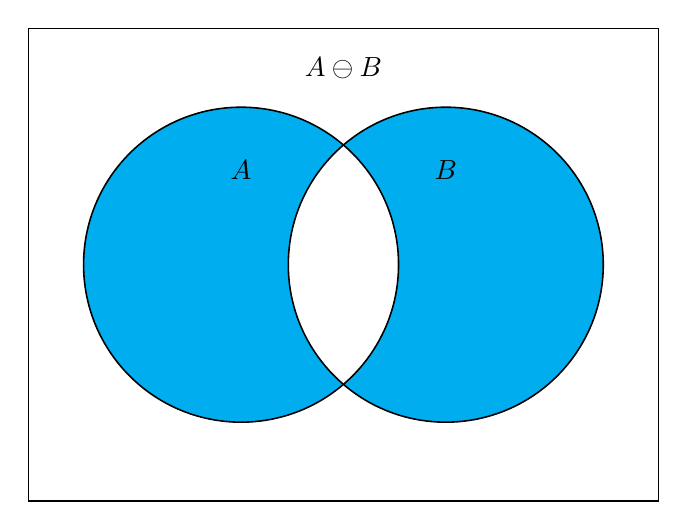
\begin{tikzpicture}[line width=0.2mm]

    % Coordinates for the centers of the circles.
    \coordinate (C1) at (-1.3, 0);
    \coordinate (C2) at ( 1.3, 0);

    % Coordinates for the labels.
    \coordinate (A) at (-1.3, 1.2);
    \coordinate (B) at ( 1.3, 1.2);
    \coordinate (S) at ( 0.0, 2.5);

    % Rectangle indicating the universe set.
    \draw (-4, -3) rectangle (4, 3);

    % Fill in the circle with cyan.
    \draw[fill=cyan, draw=none] (C1) circle (2);
    \draw[fill=cyan, draw=none] (C2) circle (2);

    % Fill in the circle with cyan.
    \draw[fill=white, draw=none] (0, -1.51987) arc(-49.46:49.46:2)
                                               arc(130.54:229.46:2);

    % Give outlines to the circles.
    \draw (C1) circle (2);
    \draw (C2) circle (2);

    % Labels.
    \node at (A) {$A$};
    \node at (B) {$B$};
    \node at (S) {$A\ominus{B}$};
\end{tikzpicture}
            \caption{Venn Diagram for Symmetric Difference}
            \label{fig:Sym_Diff_Venn_Diagram}
        \end{figure}
        The concept of set difference can then be used to define the
        concept of complement.
        Thm.~\ref{thm:Set_Difference_As_Intersection} can then be
        translated into the notation of complements as follows:
        \begin{theorem}
            If $A$, $B$, and $\Omega$ are sets,
            $A,B\subseteq\Omega$, and if $A^{C}$ is the
            complement of $A$ with respect to $\Omega$, then:
            \begin{equation}
                B\setminus{A}=B\cap{A}^{C}
            \end{equation}
        \end{theorem}
        \begin{proof}
            By the definition of complement,
            $A^{C}=\Omega\setminus{A}$.
            As $A\subseteq\Omega$ and $B\subseteq\Omega$, by
            Thm.~\ref{thm:Set_Difference_As_Intersection},
            $B\setminus{A}=B\cap(\Omega\setminus{A})$,
            and therefore $B\setminus{A}=B\cap{A}^{C}$.
        \end{proof}
        The main result about complements are known as
        DeMorgan's Laws. The laws relate unions and
        intersections by means of complements. The general
        laws hold for arbitrary unions and arbitrary
        intersections, as will be shown later.
        \begin{ftheorem}{DeMorgan's Laws}{DeMorgans_Law}
            If $A$, $B$, and $\Omega$ are sets, if
            $A\subseteq\Omega$ and $B\subseteq\Omega$, then:
            \begin{subequations}
                \begin{align}
                    \big(A\cap{B}\big)^{C}
                    &=A^{C}\cup{B}^{C}\\
                    \big(A\cup{B}\big)^{C}
                    &=A^{C}\cap{B}^{C}
                \end{align}
            \end{subequations}
        \end{ftheorem}
        With this, we can prove some results about
        set differences.
        \begin{theorem}
            If $A$ and $B$ are sets, then:
            \begin{equation}
                A=\big(A\cap{B}\big)
                    \cup\big(A\setminus{B}\big)
            \end{equation}
        \end{theorem}
        \begin{proof}
            For let $\Omega=A\cup{B}$. Then
            $A\subseteq\Omega$ and $B\subseteq\Omega$,
            and thus:
            \begin{subequations}
                \begin{align}
                    \big(A\cap{B})\cup\big(A\setminus{B}\big)
                    &=\big(A\cap{B}\big)
                        \cup\big(A\cap{B}^{C}\big)\\
                    &=A\cap(B\cup{B}^{C})\\
                    &=A\cap\Omega
                \end{align}
            \end{subequations}
            But by Thm.~\ref{thm:Intersection_is_Smaller_Left},
            $A\cap\Omega=A$. Therefore, etc.
        \end{proof}
        \begin{theorem}
            If $A$, $B$, and $C$ are sets, then:
            \begin{equation}
                A\cap\big(B\setminus{C}\big)
                =\big(A\cap{B}\big)\cap\big(A\setminus{C}\big)
            \end{equation}
        \end{theorem}
        \begin{proof}
            For:
            \begin{subequations}
                \begin{align}
                    A\cap\big(B\setminus{C}\big)
                    &=A\cap\big(B\cap{C}^{C}\big)\\
                    &=\big(A\cap{A}\big)
                        \cap\big(B\cap{C}^{C}\big)\\
                    &=\big(A\cap{B}\big)
                        \cap\big(A\cap{C}^{C}\big)\\
                    &=\big(A\cap{B}\big)
                        \cap\big(A\setminus{C}\big)
                \end{align}
            \end{subequations}
        \end{proof}
        Intersections do distribute over set differences.
        \begin{theorem}
            If $A$, $B$, and $C$ are sets, then:
            \begin{equation}
                A\cap(B\setminus{C})=
                (A\cap{B})\setminus(A\cap{C})
            \end{equation}
        \end{theorem}
        \begin{proof}
            For:
            \begin{subequations}
                \begin{align}
                    \big(A\cap{B}\big)\setminus
                        \big(A\cap{C}\big)
                    &=\big(A\cap{B}\big)
                        \cap\big(A\cap{C}\big)^{C}\\
                    &=\big(A\cap{B}\big)
                        \cap\big(A^{C}\cup{C}^{C}\big)\\
                    &=\big[\big(A\cap{B}\big)\cap{A}^{C}\big]
                        \cup\big[\big({A}\cap{B}\big)
                        \cap{C}^{C}\big]\\
                    &=\big[\big(A\cap{A}^{C}\big)\cap{B}\big]
                        \cup\big[\big(A\cap{B}\big)
                        \cap{C}^{C}\big]\\
                    &=\emptyset\cup\big[\big(A\cap{B}\big)
                        \cap{C}^{C}\big]\\
                    &=\big(A\cap{B}\big)\cap{C}^{C}\\
                    &=A\cap\big(B\cap{C}^{C}\big)\\
                    &=A\cap\big(B\setminus{C}\big)
                \end{align}
            \end{subequations}
            Therefore, etc.
        \end{proof}
        Unions do not, however. For let $A$ be non-empty
        and let $A=B=C$. Then $A\cup(B\setminus{C})=A$, but
        $(A\cup{B})\setminus(A\cup{C})=\emptyset$.
        \begin{theorem}
            If $A$ and $B$ are sets and $A\subset B$,
            then $B\setminus(B\setminus A)=A$.
        \end{theorem}
        \begin{proof}
            For:
            \begin{align}
                Yo
            \end{align}
            $[x\in B\setminus(B\setminus{A})]%
            \Rightarrow[x\in{B}\land{x}\notin%
            \{x\in{B}:x\notin{A}\}]%
            \Rightarrow[x\in{A}\subset{B}]$.
            $[x\in{A}]\Rightarrow[x\notin{B}\setminus{A}]%
            \Rightarrow[x\in{B}\setminus(B\setminus{A})]$.
        \end{proof}
        The previous theorem shows that $(A^C)^{C}=A$.
        % Untrue garbage.
        % If $A$ and $B$ are sets, and if $C\subseteq{A}\cup{B}$, then
        % either $C\subseteq{A}$ or $C\subseteq{B}$, or both. It is
        % possible that $C\subseteq{A}\cup{B}$ and yet $C$ and $B$ have no
        % elements in common, as long as $C\subseteq{A}$. As an example,
        % take $A$ and $B$ to be disjoint sets. Then $A\subseteq{A}\cup{B}$,
        % yet $A$ and $B$ have no elements in common. If
        % $C\subseteq{A}\cap{B}$, then it must be true that
        % $C\subseteq{A}$ and $C\subseteq{B}$.
        % As with the notions of unions and intersections, set differences and
        % symmetric differences can be visualized using Venn diagrams.
        \begin{theorem}
            \label{thm:MEASURE_THEORY_SET_DIFFERENCE_AS_INTERSECTION}
            If $A$, $B$, and $C$ are sets, and if $A\subseteq{C}$
            and $B\subseteq{C}$, then:
            \begin{equation}
                B\setminus{A}=B\cap(C\setminus{A})
            \end{equation}
        \end{theorem}
        \begin{proof}
            For if $x\in{B}\setminus{A}$, then
            $x\in{B}$ and $x\notin{A}$. But
            $B\subseteq{C}$, and thus if $x\in{B}$, then $x\in{C}$.
            But if $x\notin{A}$, then $x\in{C}\setminus{A}$. Therefore
            $B\setminus{A}\subseteq{B}\cap(C\setminus{A})$.
            Similarly, $B\cap(C\setminus{A})\subseteq{B}\setminus{A}$,
            and therefore $B\setminus{A}={B}\cap(C\setminus{A})$.
        \end{proof}
        While set difference appears similar to subtraction that one finds in
        basic arithmetic, the two have their differences. For any two real
        numbers $a$ and $b$, $b=a-(a-b)$. For sets this is not true. For let $A$
        be the empty set, and let $B$ be non-empty. Then
        $A\setminus(A\setminus{B})=\emptyset$, which is not $B$.
        Also, while it may seems convincing that
        $A\setminus(B\setminus{A})=A\setminus{B}$, this is not true. For
        let $A$ be a non-empty set and let $B=A$. Then
        $A\setminus(B\setminus{A})=A$, but $A\setminus{B}=\emptyset$.
        The concept of set difference can then be used to define the
        concept of complement.